\subsection{Kryptografické algoritmy a protokoly}

\begin{obecne}{Cíle kryptografie}
  \begin{pitemize}
    \item důvěrnost dat
    \item celistvost dat
    \item autentifikace~-- od koho jsou data
    \item nepopiratelnost~-- když jednou něco potvrdím, nemohu to popřít.
  \end{pitemize}
\end{obecne}

\begin{definiceN}{Kryptografický systém}
 \textbf{ Kryptografický systém} obsahuje:
  \begin{pitemize}
    \item prostor zpráv~-- \emph{plaintext},
    \item prostor šifrovaných zpráv~-- \emph{ciphertext},
    \item prostory šifrovacích a dešifrovacích \emph{klíčů},
    \item efektivní algoritmus pro \emph{generování klíčů},
    \item efektivní algoritmus pro \emph{šifrování},
    \item efektivní algoritmus pro \emph{dešifrování}.
  \end{pitemize}
\end{definiceN}

\begin{definiceN}{označení}
  $C$~-- šifra, $P$~-- otevřený text, $K$~-- klíč,\\
  $\mathbf{E}$~-- šifrovací algoritmus, $\mathbf{D}$~-- dešifrovací algoritmus.\\[3mm]
  \emph{Šifrování:} $C = \mathbf{E}(P)$, resp. $C = \mathbf{E}(K, P)$\\
  \emph{Dešifrování:} $P = \mathbf{D}(C)$, resp. $P = \mathbf{D}(K, C)$\\
\end{definiceN}


\begin{obecne}{Kerchoffovy principy dobrého krypt. systému}
\begin{pitemize}
    \item E a D neobs. tajnou část
    \item E distribuuje rozumné zprávy rovnoměrně po C
    \item se správným klíčem jsou E \& D efektivní
    \item bez správného klíče je dešifrování minimáně NP-úplné. 
\end{pitemize}
\end{obecne}

\begin{obecne}{dělení kryptografických systémů}
\begin{pitemize}
    \item symetrické krypt. systémy : $k = k'$
    \item asymetrické : $k \neq k'$ ( veřejný a tajný klíč ). 
\end{pitemize}
\end{obecne}

\begin{obecne}{Model útočníka podle Doleva a Yao}
\begin{pitemize}
    \item může získat jakokoliv zprávu jdoucí po síti, může zahájit komunikaci s jiným uživatelem, může se stát příjemcem zpráv od kohokoliv, může zasílat zprávy komukoliv \& vydávat se za jiného uživatele, 
    \item nemůže uhádnout náh. číslo z dost velké množiny, bez klíče nemůže dešifrovat zprávu \& nemůže vytvořit platnou šifrovanou zprávu (vzhledem k šifr. alg.).
\end{pitemize}
\end{obecne}

\subsubsection*{Kryptografické protokoly}

\begin{pitemize}
   \item \textbf{Arbitrované protokoly}~-- rozhodčí dělá skoro všechno.
   \item \textbf{Rozhodované protokoly}~-- rozhodčí je dobrý jenom při sporu aby rozhodl.
   \item \textbf{Samozabezpečovací protokoly}~-- není žádná třetí strana.
\end{pitemize}

\begin{obecne}{Anonymní platby}
  Problém kreditních karet spočívá v sledovatelnosti toku peněz. Hledáme protokol
  pro tvorbu autentizovaných ale nesledovatelných zpráv.
\end{obecne}

\begin{obecne}{Časové známky}
  Nejjednodušší metodou je zasílat kopie zpráv důvěryhodnému arbitrovi, problémy s
  množstvím uchovávaných dat lze vyřešit použitím hašovacích funkcí.

  Používají se spojené (linked) aby odesílatel spolu s arbitrem nemohli podvádět.
  \begin{penumerate}
    \item Odesílatel $S$ zašle arbitrovi $A$ hashkod zprávy $H_n$.
    \item $A$ vrátí odesílateli 
    $T_n=S_K(n,S,H_n,Tm_n;Id_{n-1},H_{n-1},T_{n-1},H(Id_{n-1},H_{n-1},T_{n-1}))$
    kde $n$ je pořadí zprávy, $Tm_n$ čas podpisu zprávy, $Id_{n-1}\ldots$ jsou informace
    o předešlé zprávě, kterou arbitr vyřizoval.
    \item Po vyřízení následující zprávy arbitr zašle odesílateli identifikaci
    následujícího odesilatele
  \end{penumerate}
  Chce-li někdo ověřit časovou známku zprávy, kontaktuje odesilatele $Id_{n-1}$ a
  $Id_{n+1}$ a pomoci nich ověří platnost $T_n$
\end{obecne}

\begin{obecne}{Digitální podpisy}
  Musí být nefalšovatelné, autentické, neměnitelné, \uv{nerecyklovatelné}.
  \paragraph{Symetrické systémy:}
   Nechť odesílatel $S$ zasílá příjemci $R$ zprávu $M$
   \begin{penumerate}
      \item $S$ zašle arbitrovi $A$ zprávu $\mathbf{E}(M,K_S)$.
      \item Arbitr verifikuje odesílatele a příjemci $R$ zašle 
      $\mathbf{E}((M,S, \mathbf{E}(M,K_S)),K_R)$
      \item Příjemce uchová $M$ a $\mathbf{E}(M,K_S)$ pro účely případného dokazování přijetí.
   \end{penumerate}

   \paragraph{Asymetrické systémy:}
   Stačí provést $\mathbf{E}(\mathbf{D}(M,K_S),K_R)$

\end{obecne}

\begin{obecne}{Důkazy s nulovou znalostí}
  \begin{pitemize}
    \item dokazovatel nesmí podvádět - pokud důkaz nezná, jeho šance přesvedčit arbitra
    je mizivá
    \item ověřovatel nesmí podvádět - o důkazu smí zjistit jenom to, ze ho dokazovatel zná.
    V žádném případě nesmí být schopen důkaz zrekonstruovat a sám provést.
    \item ověřovatel se nesmí dozvědět nic, co by nebyl schopen zjistit bez pomoci 
    dokazovatele.
  \end{pitemize}
  Není-li splněna poslední podmínka mluvíme o \emph{důkazech s minimálním vyzrazením}.
  Jeden z možných důkazů je založen na problematice Hamiltonovských kružnic v grafu.
  \begin{penumerate}
    \item Nechť $A$ zná Hamiltonovskou kružnici v grafu $G$.
    \item $A$ provede náhodnou permutaci očíslování vrcholů $G$. Původní graf a vzniklý $H$ jsou izomorfní.
    \item Kopie grafu $H$ je zaslána entitě $B$.
    \item Ověřovatel $B$ položí dokazovateli $A$ jednu z následujících otázek
    \begin{penumerate}
	\item Dokázat, že $G$ a $H$ jsou izomorfní
	\item Ukázat Hamiltonovskou kružnici v grafu $H$
    \end{penumerate}
    \item Opakováním kroku 1. až 4. lze docílit potřebné jistoty. 
  \end{penumerate}
\end{obecne}

\begin{obecne}{Neurčitý obnos (Oblivious transfer)}
  Protokol umožňuje, aby si adresát vybral z několika nabízených možností aniž
  by odesílatel předem znal jeho volbu, možné doplnění o následnou vzájemnou
  kontrolu.
\end{obecne}

\begin{obecne}{Podepisování kontraktů (Contract signing)}
  V každém okamžiku musí být obě smluvní strany vázány stejně moc.
  Nejjednodušším řešením je arbitrovaný protokol, kde obě strany předají
  centrální autoritě své podepsané kopie a tato třetí strana zajistí výměnu po
  obdržení obou kopií.
\end{obecne}

\begin{obecne}{Elektronická potvrzovaná pošta (digital certified mail)}
  Chceme, aby adresát mohl přečíst naši zprávu až poté, co získáme potvrzení o
  tom, že ji obdržel (elektronický doporučený dopis).
\end{obecne}

\begin{obecne}{Bezpečné volby}
  \begin{pitemize}
    \item volit smí pouze oprávnění voliči,
    \item každý smí hlasovat nejvýše jednou,
    \item nikdo nesmí vědět, kdo jak volil,
    \item nikdo nesmí měnit volbu jiných,
    \item každý hlas musí být započítán.
  \end{pitemize}

  Nejjednodušší možnost je použít protokol se dvěmi centrálními autoritami.
  Používá registrační autoritu $RA$ provádějící registraci voličů a sčítací
  autoritu $SA$, která sčítá hlasovací lístky a zveřejňuje výsledky voleb.
  \begin{penumerate}
    \item Všichni voliči zašlou $RA$ žádost o validační číslo.
    \item $RA$ zašle každému voliči náhodně zvolené validační číslo $L$ a zároveň
    si poznamená kdo jaké číslo dostal.
    \item $RA$ zašle seznam validačních čísel $SA$.
    \item Kazdy z voličů si náhodně vybere svoje identifikační číslo $Id$ a $SA$
    zašle zprávu $(L, Id, v)$ kde v je jeho volba.
    \item $SA$ porovná $L$ se seznamem validačních čísel z kroku 3. Odpovídající
    číslo škrtne a voličovo $Id$ přidá do seznamu asociovaného s voleným kandidátem.
    \item Po skončení voleb $SA$ zveřejní výsledky a seznamy identifikačních čísel
    spojené se jmény kandidátů.
  \end{penumerate}
\end{obecne}

\begin{obecne}{Útoky na protokoly}
  \begin{pitemize}
    \item \emph{přehrání zpráv}~-- M odposlouchá všechny zprávy a pak totéž udělá sám
    \item \emph{muž uprostřed} (man-in-the-middle)
    \item \emph{paralelní spojení}~-- několik běhů protokolů prováděných současně pod
    řízením M
    \item \emph{odražení}~-- A zahájí komunikaci, M zachytí zprávu, upraví ji, aby
    nebyl poznat původní A a pošle ji zpět A
    \item \emph{prokládání}~-- Několik běhů protokolu prováděných současně pod
    řízením M, zprávy z jednoho se použijí u dalšího, atd.
    \item \emph{chyba typu}~-- Nedodržení přesného sémantického významu zprávy
    \item \emph{vypuštění jména}~-- Pokud v protokolu není poznat, kdo za to může
    \item \emph{chybné použití šifrovací služby}~-- Špatný algoritmus použitý na nevhodném místě
  \end{pitemize}
\end{obecne}

\subsubsection*{Kryptografické algoritmy}

\begin{definiceN}{Substitution-box~-- S-box}
  \begin{pitemize}
    \item krabička která z \emph{m} bitů vstupu dělá \emph{n} bitů výstupu.
    \item někdy je použita pevná tabulka. Např. u DES
    \item někdy je výstup s-boxu závislý na klíči. Např. u Blowfish, Twofish
    \item v blokových šifrách je to často s-box kdo zamlžuje vztah mezi plaintextem a šifrou.
    \item dost často na něm závisí jak je šifra napadnutelná $\Rightarrow$ musí
    se volit dost obezřetně
  \end{pitemize}
\end{definiceN}

\begin{obecne}{Symetrické}
  \begin{pitemize}
    \item vysoká datová propustnost
    \item klíče na obou koncích musí zůstat utajeny $\Rightarrow$ je třeba často
    měnit klíče
    \item potřeba ověřené TTP (Trusted Third Party)
  \end{pitemize}
\end{obecne}

\begin{obecne}{DES}
  Vyvinula firma IBM na zakázku NBS počátkem 70. let. Původní název DEA, v USA
  DEA1. Jako standard přijat 23. 11. 1976 Dodnes používán v komerční sféře, pro
  vojenské účely není certifikován ani pro ochranu neklasifikovaných informací.
  Patrně nejrozsáhleji používaný šifrovací algoritmus všech dob.

  Šifruje 64-bitové bloky otevřeného textu na 64-bitové výstupní bloky, délka
  klíče 64 bitů.

  \begin{figure}[!ht]
    \begin{center}
      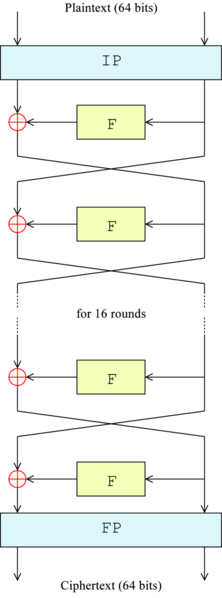
\includegraphics[scale=.7, angle=90]{informatika/algoritmy_a_ds/obrazky/DES-main-network.png}
      \caption{Struktura hlavní sítě algoritmu DES (zdroj: Wikipedie)}
    \end{center}
  \end{figure}

  \paragraph{Analýza:}
  \begin{pitemize}
    \item velká slabina je 64-bitový klíč (navíc efektivně pouze 56-bitový).
    Prolomen za méně než 24 hodin.
    \item úvodní permutace nemá prakticky žádný vliv
    \item existence slabých $(\mathbf{E}(K)=\mathbf{D}(K))$ a poloslabých
    $(\mathbf{E}(K_1)\mathbf{E}(K_2)=Id.)$ klíčů
    \item komplementárnost $C=\mathbf{E}(K,P)\Leftrightarrow\lnot C= \lnot
    \mathbf{E} (\lnot K,\lnot P)$
  \end{pitemize}
\end{obecne}

\begin{obecne}{Blowfish}
  \begin{pitemize}
    \item nástupce systému DES, 
    \item opět Feistelova šifra, délka bloku je 64 bitů, proměnná délka klíče až 448 bitů
    \item algoritmus provádí 16 cyklů nad vstupem délky 64-bitů
  \end{pitemize}
\end{obecne}

\begin{obecne}{IDEA}
  \begin{pitemize}
    \item z roku 1991, vyšel pod názvem IPES. 
    \item IDEA (International Data Encryption Algorithm)
    \item bloková šifra s délkou bloku 64-bitů a délkou klíče 128-bitu
    \item algoritmus je patentován 
    \item zajímavé je že pokud bychom algoritmus upravili tak, že bychom všechny řetězce
    se kterými pracuje zvětšili na dvojnásobek, tak dojde ke ztrátě bezpečnosti.
    \item algoritmus je považován za bezpečný.
  \end{pitemize}
\end{obecne}

\begin{obecne}{RC5}
  \begin{pitemize}
    \item z roku 1994 od R. Rivesta
    \item používá rotace závislé na datech.
    \item algoritmus umožňuje nastavit spoustu parametrů:
    \begin{pitemize}
      \item délka šifrovacího klíče (0\dots255 bytů)
      \item počet kol šifrovacího procesu (0\dots255)
      \item z hodnot 16, 32, 64, ale i vyšších lze zvolit délku slova, algoritmus
      zpracovává bloky o délce dvojnásobku slova
    \end{pitemize}
  \end{pitemize}

\end{obecne}

\begin{obecne}{Kryptosystém Rijndael}
  \begin{pitemize}
    \item produkční bloková šifra
    \item proměnná délka bloku~-- 16, 24 nebo 32 bajtů
    \item proměnná délka klíče~-- 128, 192 nebo 256 bitů
  \end{pitemize}

  \paragraph{Analýza:} Po rozsáhlé analýze nenalezena žádná slabina a tak
  zvolen jako nový standard AES.
\end{obecne}

\begin{obecne}{RC4}
  \begin{pitemize}
    \item proudová šifra od R. Rivesta
    \item jednoduchý a rychlý algoritmus 

    \paragraph{Analýza:} Zatím není známý žádný způsob útoku $\Rightarrow$
    algoritmus považován za bezpečný.
  \end{pitemize}
\end{obecne}

\begin{obecne}{FISH}
  \begin{pitemize}
    \item proudová šifra založena na Fibonacciho generátoru pseudonáhodných čísel.
    \item z fibonacciho generátoru se získá posloupnost a šifrovaní se provádí
    například XORováním této posloupnosti s \emph{P}
  \end{pitemize}
\end{obecne}

\begin{obecne}{Asymetrické}
  \begin{pitemize}
    \item šifry s asymetrickým klíčem~-- RSA, DSA (ElGammal)
    \item mnohem pomalejší
    \item není potřeba TTP
    \item pouze jeden klíč tajný, nemusí se měnit tak často
    \item o žádném schématu veřejného klíče nebylo dokázáno, že je bezpečné
  \end{pitemize}
\end{obecne}

\begin{obecne}{RSA}
  Kryptoschéma je založeno na Eulerově formuli: 
  $$a^{\varphi(n)} \equiv 1(mod\ n)$$ 
  kde $\varphi(n)$ je počet čísel z intervalu $1..n$ která jsou s $n$ nesoudělná.

  \paragraph{Šifrování:} Je třeba znát číslo $n$ a malé prvočíslo $e$. Otevřený
  text převedeme do posloupnosti modulo $n$. Každý blok $P_j$ zašifrujeme dle
  vzorce: $$C_j\equiv P_j^e\ (mod\ n)$$ Spojením výsledných bloků vznikne
  zašifrovaný text.

  \paragraph{Dešifrování:} Je třeba znát číslo $n$ a číslo $d$. Každý z bloků
  potom dešifrujeme takto: $$P_j\equiv C_j^d\ (mod\ n)$$ Pro dešifrovací klíč
  $d$ musí platit: $$ed\equiv 1\,(mod\ \varphi(n))$$ Prvočíslo $e$ nesmí dělit
  $\varphi(n)$. $d$ určíme z předchozího vztahu rozšířeným eukleidovým
  algoritmem.

  Veřejný klíč tvoří pár $(n, e)$, soukromý klíč pár $(n, d)$. Číslo $n$ musí být velmi
  velké a nesmí mít malé faktory. Pro reálné použití 100 až 200 bitů. Hranice bezpečnosti
  1024 bitů modulu $n$, rozumné 1500 bitů, lépe 2048 bitů.

  Není známa žádná metoda vedoucí k rozbití algoritmu RSA. 
\end{obecne}

\begin{obecne}{Merkle-Hellman kryptosystém}
  \begin{pitemize}
    \item založen na problému batohu
    \item plaintext je chápán jako posloupnost vah (řešení)
    \item ciphertext je výsledná hmotnost batohu
    \item pro superrostoucí posloupnost je problém řešitelný v lineárním čase
    \item superrostoucí posloupnost je součást soukromého klíče a tak
    dešifrování pomocí ní je zvládnutelné lineárně, kdežto bez ní je to NP-úplný
    problém
    \item systém byl prolomen! Není tedy považován za bezpečný. Útočník je
    schopen získat superrostoucí posloupnost a pomocí ní může dešifrovat
  \end{pitemize}
\end{obecne}

\begin{obecne}{Elgamal kryptosystém}
  Založen na obtížnosti výpočtu diskrétního logaritmu nad kruhem.

  Potřebujeme společný modul $q$ a číslo $g$ co nejvyššího řádu. Každý účastník si zvolí tajný
  klíč $y_i$ a vypočítá veřejný klíč $g^{y_i}$ mod $q$.
  \paragraph{Šifrování:} Nechť uživatel \emph{A} posílá zprávu \emph{P}
  uživateli \emph{B}. Náhodně
  vybere číslo $k$ a vypočítá: $$ g^k \mod q;\ P \otimes{(g^{y_b})}^k \mod q
  $$ obě čísla zašle \emph{B}.

  \paragraph{Dešifrování:} Uživatel \emph{B} vypočítá: $$ {(g^k)}^{y_b} \mod q$$
  a najde inverzní prvek. Z druhého čísla potom snadno získá \emph{P}.

  Systém je považován za bezpečný. Nevýhodou je nutnost generovat náhodné číslo
  $k$ a zdvojnásobení dat během šifrování.
\end{obecne}
